\section{Sequential GF Multiplier Design}
\label{sec:design}

Let us briefly describe the fundamentals behind the design of normal
basis sequential GF multipliers, so as to put in perspective the type
of designs that have been verified in this paper. Let $R =
\sum_{i=0}^{k-1} r_i \beta^{2^{i}}, ~A = \sum_{i=0}^{k-1} a_i
\beta^{2^{i}}, ~B = \sum_{i=0}^{k-1} b_i \beta^{2^{i}}$, then 
\[
R = A\cdot B = (\sum_{i=0}^{k-1} a_i \beta^{2^{i}}) (\sum_{j=0}^{k-1}
b_j \beta^{2^{j}})  =
\sum_{i=0}^{k-1}\sum_{j=0}^{k-1}a_ib_j\beta^{2^i}\beta^{2^j}\nonumber 
\]

The expressions $\beta^{2^i}\beta^{2^j}$ are called cross-product
terms and they can also be represented in normal basis: 
\begin{displaymath}
\beta^{2^i}\beta^{2^j} =
\sum_{n=0}^{k-1}\lambda_{ij}^{(n)}\beta^{2^n}, \ \ \lambda_{ij}^{(n)}
\in \Ftwo. 
\end{displaymath}

From the above two equations, one can see that the expression for the
$n^{th}$ digit of product $R = (r_0, \dots, r_n, \dots r_{k-1})$ is:
\[
r_n = \sum_{i=0}^{k-1}\sum_{j=0}^{k-1}\lambda_{ij}^{(n)}a_ib_j = A
\cdot M_n \cdot B^T, ~~0 \leq n \leq k-1
\]

where $M_n = (\lambda_{ij}^{(n)})$ is a binary $k \times k$ matrix over
$\Ftwo$, and it is called the $\lambda$-matrix. 
%The collection of all
%$\{M_n\}$  $\lambda$-matrices is called the multiplication
%table. 
Moreover, let $r_n = A \cdot M^{(n)} \cdot B^T$.
Then $r_{n-1} = A \cdot M^{(n-1)} \cdot B^T = rotate(A) \cdot M^{(n)}
\cdot rotate(B)^T$. This implies that $M^{(n)}$ is generated by right
and down cyclic shifting $M^{(n-1)}$. Therefore, the hardware design
of sequential GF multipliers is based on mappings of $A\cdot M_n
\cdot B^T$ into AND-XOR gates and cyclic shift operations. 

This paper verifies the implementation of two distinct 
architectures of {\it sequential multipliers with parallel output
  (SMPO)}, namely: i) the Agnew-SMPO  \cite{agnew1991implementation}
by G. B. Agnew, which is a straight-forward implementation of the
$\lambda$-matrix; and ii) the more recent, more complicated, yet very
efficient RH-SMPO \cite{RHmulti}, by Reyhani-Masoleh and Hasan,
depicted in Fig. \ref{fig:RHmulti}.  

\begin{figure}[hbt]
\centering{
%\begin{minipage}{12cm}
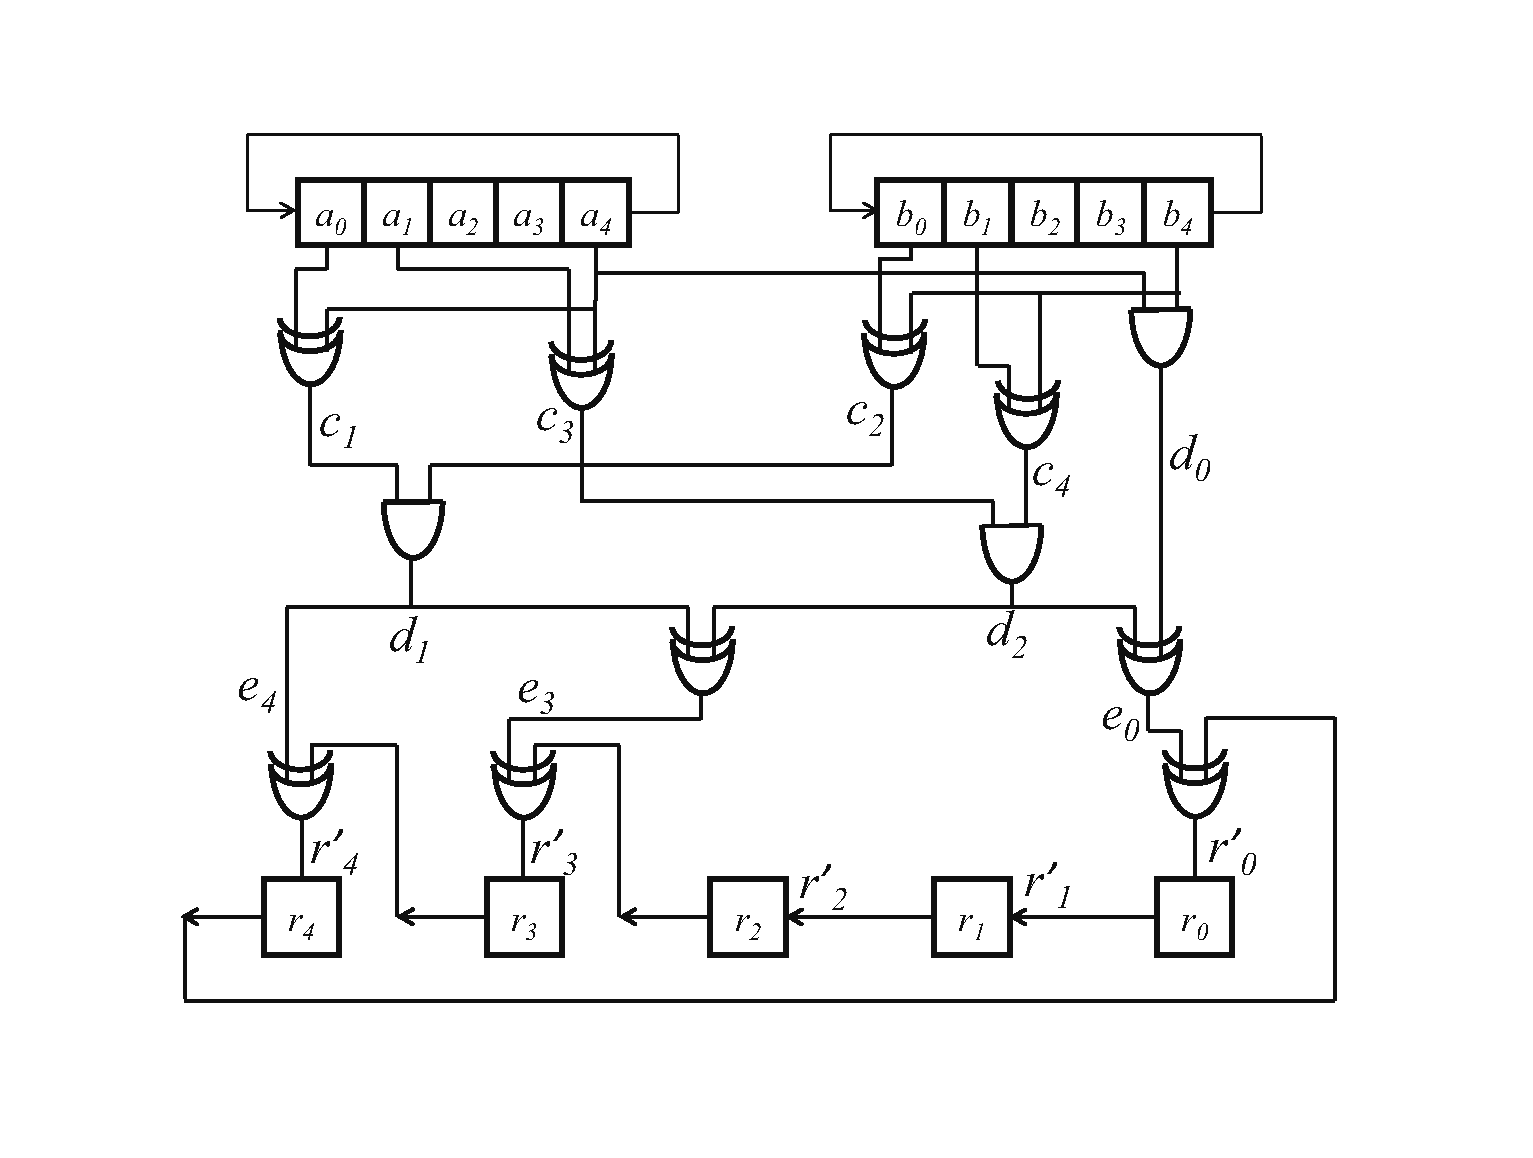
\includegraphics[width=4in]{./RH.eps}
\vspace{-0.2in}
\caption{A 5-bit Reyhani-Hasan Sequential Multiplier with Parallel Outputs (RH SMPO)}
%\end{minipage}
\label{fig:RHmulti}}
\end{figure}
